\section{Introduction}\label{sec:introduction}
% ---------------------------------------------
% goal: draw a picture of the context in which your work is embedded.

In the introduction, get the attention of the reader and draw a picture of the context in which your work is embedded. This should include:

\begin{itemize}
    \item Motivation: Describe the ultimate goal, the glory future that we want to reach.
    \item Problem Statement: Why is there currently a gap between us and our goal? What is the problem?
    \item Contributions: What will you do / have you done to narrow this gap?
\end{itemize}

For example, start with an interesting statistic:
Road intersections are not only a hot spot for accidents but also cause delays and congestions, especially in urban areas.
According to \cite{stau}, drivers in the US spend an additional 100 hours per year in their vehicles due to congestion and these delays have caused additional costs of 88 billion USD in 2019.





\subsection{Contributions}\label{sec:contributions}
Your contributions are of high interest to the reader. It is good practice to give them their own subsection to be easily spotted. In the best case this subsection is still visible on the first page.
Provide a short list of contributions that this paper provides and add forward references to the sections where they covered. 

For example: This paper addresses the scheduling problem for intersections and the required communication on an architectural level. We assume that once the vehicles have agreed on a schedule for crossing the intersection, they can execute a safe crossing autonomously.

In particular, we
\begin{itemize}
    \item propose a distributed intersection management scheme which uses consensus to agree on schedule groups (\cref{sec:approach}),%(\sectionref{sec:approach}).
    \item provide a \texttt{C++} implementation for the realistic simulation framework SUMO (\cref{sec:details}),
    \item discuss related approaches from literature and why they are over-optimistic (\cref{sec:related}),
    % (\sectionref{sec:sota})
    \item simulate and evaluate safety and delay (\cref{sec:evaluation}).
\end{itemize}



	% ===================================================
	\newcommand\circnum[1]{\textcolor{col_prim}{\textcircled{\raisebox{-0.9pt}{#1}}}}
	\begin{figure}[t]
	  \centering
	  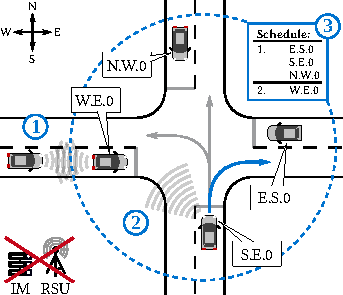
\includegraphics[width=\columnwidth]{res/img/idea}
	  \caption{Example Image of the main idea: Vehicles agree P2P on schedule groups using three communication phases: \circnum{1} Intra-Lane Exchange, \circnum{2} Inter-Lane Exchange, and \circnum{3} Schedule Group Consensus. No central Intersection Managers (IM) or Road-Side Units (RSU) are required.}
	  \label{fig:idea}
	\end{figure}
	% ===================================================

